\documentclass[12pt]{article}%
\usepackage{fancyhdr}
\usepackage{hyperref}
\usepackage[a4paper, margin=0.95in]{geometry}
\usepackage{common-math}

\begin{document}

\title{Final Report\\ \vspace{0.1in}
\Large Dirichlet Domains and Deformations of\\
Convex Projective Structures}
\author{John Teague}
\maketitle

\section{Background}

This project arose out of a research problem I am thinking about under the guidance of a professor in the math department, Dr. Jeffrey Danciger. It falls loosely into the subject of \textit{geometric topology}.


There is a deep idea in mathematics that the geometry of a space can be encoded by the symmetries of that space that preserve the geometry. This goes back to Klein, with his Erlangen program. The idea is to define geometry by an abstract characterization of the symmetries of that geometry, called the \textit{isometry group}. For example, 
\begin{itemize}
	\item Euclidean geometry is given by the data of the space $\R^n$ and the Euclidean isometry group $\Euc(n) = \O(n) \ltimes \R^n$, consisting of translations, rotations, and reflections.
	\begin{itemize}
		\item Think of a triangle in high school geometry. Two triangles are the same if they can be ``transformed'' into each other using the above operations.
	\end{itemize}
	\item Spherical geometry in $2$-dimensions is given on the sphere $S^2$ with isometry group $O(3)$.
	\item Hyperbolic geometry is given by hyperbolic space $\bbH^n$ with the isometry group $\PSL_2\R$.
\end{itemize}
Additionally, it's possible to ``equip'' other spaces called \textit{manifolds} with these geometries. If you glue up a square in $\R^2$ by Euclidean isometries, e.g. translation by $\begin{pmatrix} 1\\0 \end{pmatrix}$ and $\begin{pmatrix} 0\\1 \end{pmatrix}$, you get a Euclidean or flat torus \cite{ballas}.

Mathematicians, in many areas of math, study \textit{classification problems}. They seek to classify families of mathematical objects. In this case, we might want to classify all of the possible geometries we can put on manifolds or all of the unique ways to put a given geometry on a manifold. This project focuses on the latter, looking at the specific case of putting \textit{convex projective structures} on surfaces, or $2$-dimensional manifolds. These structures come from a canonical metric on properly convex domains $\Omega$ living in $\RP^d$, called the Hilbert metric $d_\Omega$.

One way to get a handle on this is via \textit{deformation theory}. The Ehressman-Thurston principle says that geometric structures are stable under small deformation. This project seeks to visualize a number of these deformations by drawing fundamental domains (like the square gluing to the torus) for actions of discrete subgroups $\Gamma \subset \PSL_3\R$ on properly convex domains $\Omega \subset \RP^2$. One way to do that is by drawing Voronoi diagrams with respect to the Hilbert metric. In the case of the unit disk, the Hilbert metric corresponds to the ordinary hyperbolic metric, so it is also of interest to draw hyperbolic Voronoi diagrams. Also, it would potentially be novel to draw bisectors in the Hilbert metric --- another goal of this project.

The research project is specifically interested in answering the question, ``when are these fundamental domains finitely sided?''\cite{du2023geometry}

\section{Accomplishments}

So far, the following are working:

\begin{enumerate}
	\item Drawing Hyperbolic geodesics.
	\begin{enumerate}
		\item This is just getting our feet wet, so to speak. It would be nice to have a fully modeled hyperbolic space, including the ability to compute distances and geodesics.
		\item This is implemented both for the Poincar\'e and Klein disk models.
	\end{enumerate}
	\item Drawing Hilbert bisectors.
	\begin{enumerate}
		\item Start with some convex domain $\Omega$ and compute the Hilbert metric $d_\Omega$ using the cross-ratio. Then given two points $x,y \in \Omega$, draw the bisector $\{z \in \Omega : d_\Omega(x,z) = d_\Omega(z,y)\}$. There were a number of design decisions to be made:
		\begin{enumerate}
			\item There are multiple ways to commute $d_\Omega$. One idea is to keep track of the attracting hyperplanes when drawing the domain and just find which two best approximate where the endpoints $a,b$ for the chord through $x,y$ would land. Ultimately, I ended up just keeping track of the boundary edges while generating $\Omega$. This is not as mathematically accurate, since the points we solve for aren't actually on the boundary, but it is a good approximation.
			\item At first, I tried the na\"ive algorithm: sample random points in the domain and compute distances, and if $d_\Omega(x,z) - d_\Omega(z,y) < \epsilon$ for some small $\epsilon$, draw them. Since it is relatively slow to compute $d_\Omega$, it turned out to be beneficial to be a bit more clever. The final project uses a box walking technique to sample points along the bisector and drawing points if the above condition is met. I also added an option to draw the boxes as gradients instead of a simple curve.
			\item It is non-trivial to define these convex domains, and the best way to do so may be to deform a discrete representation of a group $G$ into $\PSL_2\R$ into $\SL_3\R$. For example, via a bulging or earthquake deformation. This is what I ended up doing for this project. I chose to draw the bisectors on domains gotten by bulging deformations of triangle reflection groups.

			Here is how this works technically \cite{goldman}: a subgroup \[\Gamma_1 *_\Lambda \Gamma_2 \subset \PSL_{d + 1}\R\] can be deformed as follows: let $(B_t)_t \subset \PSL_{d + 1}\R$ be a path of elements starting at the identity and that commute with $\Lambda$. Then we can deform $i: \Gamma \to \PSL_{d + 1}\R$ to representations $\rho_t$ which are the identity on $\Gamma_1$ and send $\gamma_2 \in \Gamma_2$ to $B_t\gamma_2B_t^{-1}$. If $\Gamma$ divides some $\Omega$, then representations $\rho_t$ are injective, and $\rho_t(\Gamma)$ divides a properly convex domain $\Omega_t$. By the Ehresmann-Thurston principle, we have that \[\Omega_t/\rho_t(\Gamma) \approx_{\text{Diffeo}} \Omega/\Gamma\] for all $t$.

			Observe, $\rho_t$ is well-defined since $B_t$ is in the identity component of the centralizer $\calZ(\PSL_3\R)$, hence both components of the representation agree on $\Lambda$. We can construct $B_t$ as follows: $B_t = e^{tB}$ where \[B = \begin{pmatrix} -1 \\ &d \\ &&-1 \\ &&&\ddots \\ &&&&-1 \end{pmatrix}.\] The project allows you to tune this $t$, and we draw $\Omega_t$.
			\item It is also currently possible to view the fundamental domain coming from the Voronoi tessellation of the triangle reflection group I chose, but not yet under the deformation. This should be an easy thing to add \cite{gezalyan2021voronoi}.
		\end{enumerate}
	\end{enumerate}
	\item Hyperbolic Voronoi diagrams.
	\begin{enumerate}
		\item Again, there were a number of options for the implementation here. I implemented Bowyer-Watson to compute the hyperbolic Delaunay triangulation (to then compute the dual Voronoi tessellation), but ultimately wasn't able to finish debugging this for the final project. The algorithm in use currently is the naive one, but it works pretty fast up to $100$ points.
		\item This works for both the Poincar\'e and Klein models, and thanks to caching, it is very fast to switch between them.
		\item For the Voronoi diagrams with respect to the Hilbert metric, I was planning on working through \cite{gezalyan2021voronoi}.
	\end{enumerate}
\end{enumerate}

\section{Artifacts}

\begin{enumerate}
	\item Hyperbolic Geodesics
		\begin{figure}[H]
			\centering
			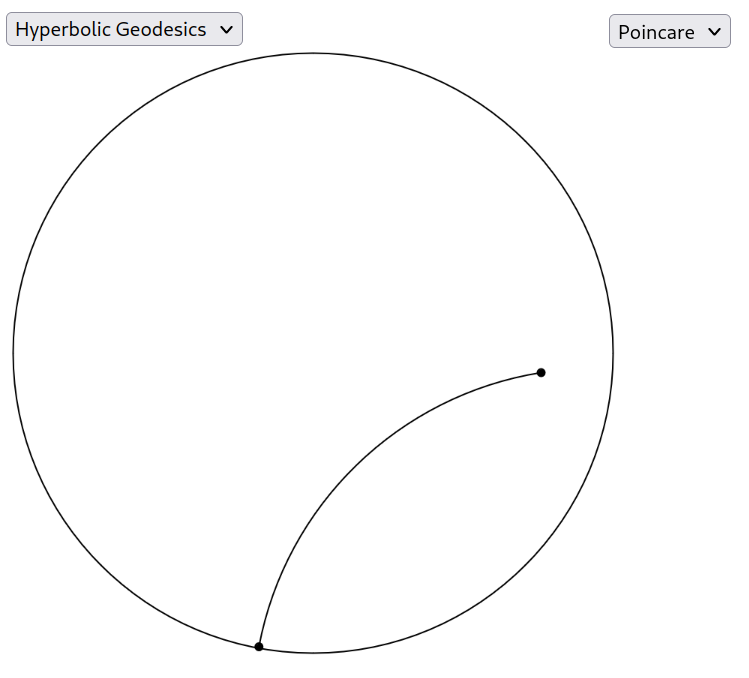
\includegraphics[scale=0.25]{p_geodesic.png}
			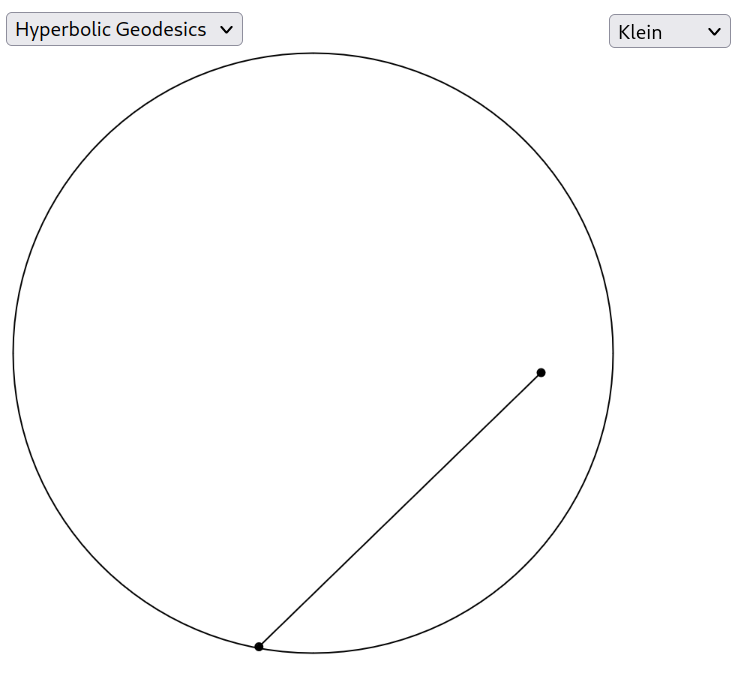
\includegraphics[scale=0.25]{k_geodesic.png}
		\end{figure}
	\item Hilbert Bisectors
		\begin{figure}[H]
			\centering
			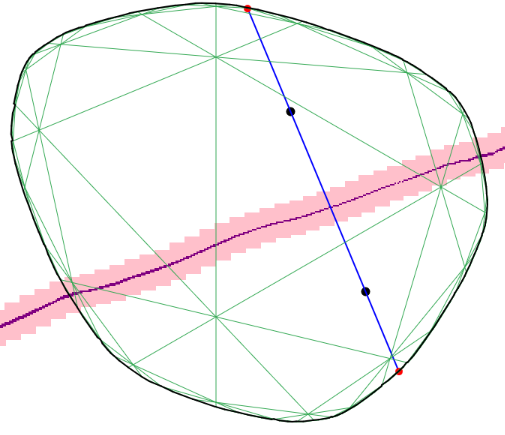
\includegraphics[scale=0.25]{mild_deformation.png}
			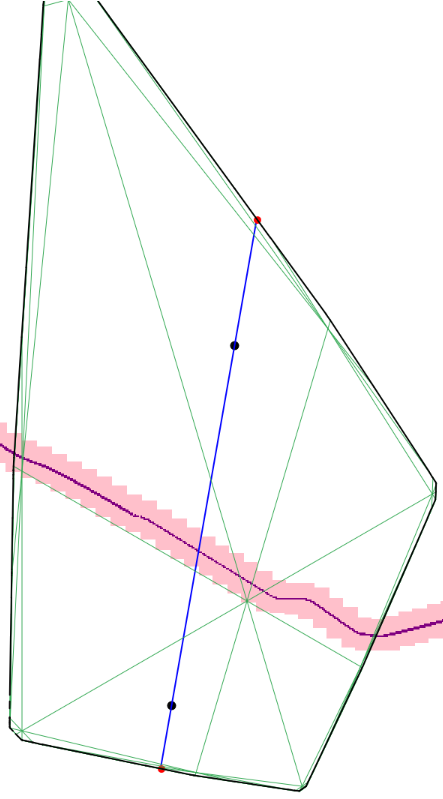
\includegraphics[scale=0.25]{extreme_deformation1.png}
			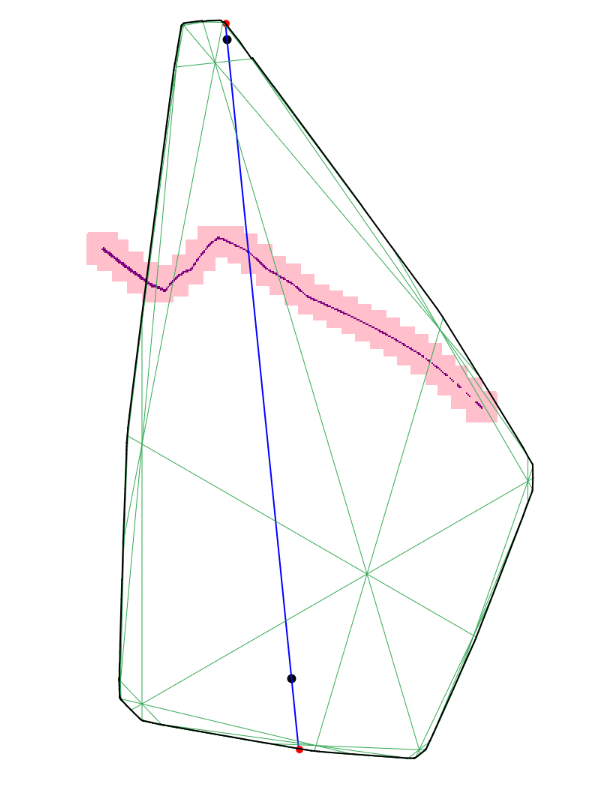
\includegraphics[scale=0.25]{extreme_deformation2.png}
		\end{figure}
		\begin{figure}[H]
			\centering
			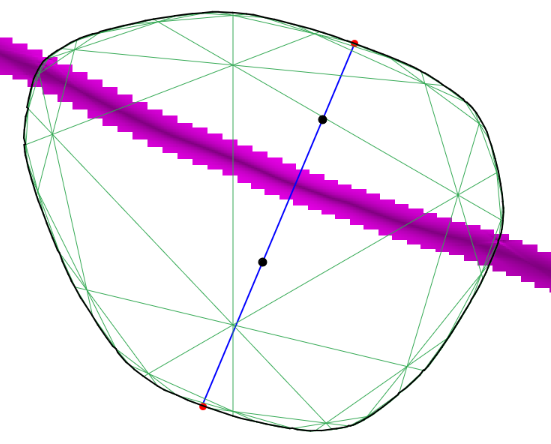
\includegraphics[scale=0.3]{gradient_bisector.png}
		\end{figure}
	\item Hyperbolic Voronoi diagrams
	\begin{figure}[H]
		\centering
		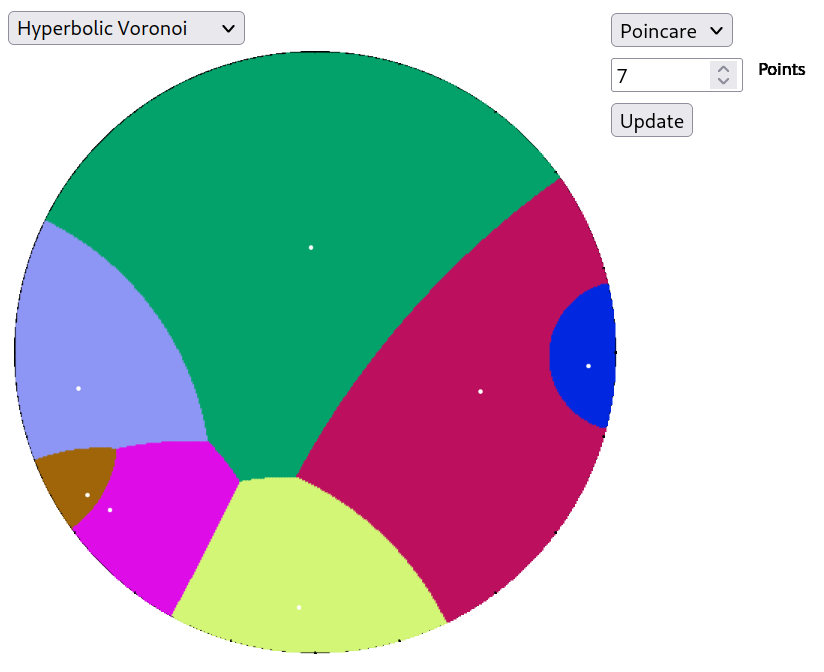
\includegraphics[scale=0.25]{p_voronoi_small.png}
		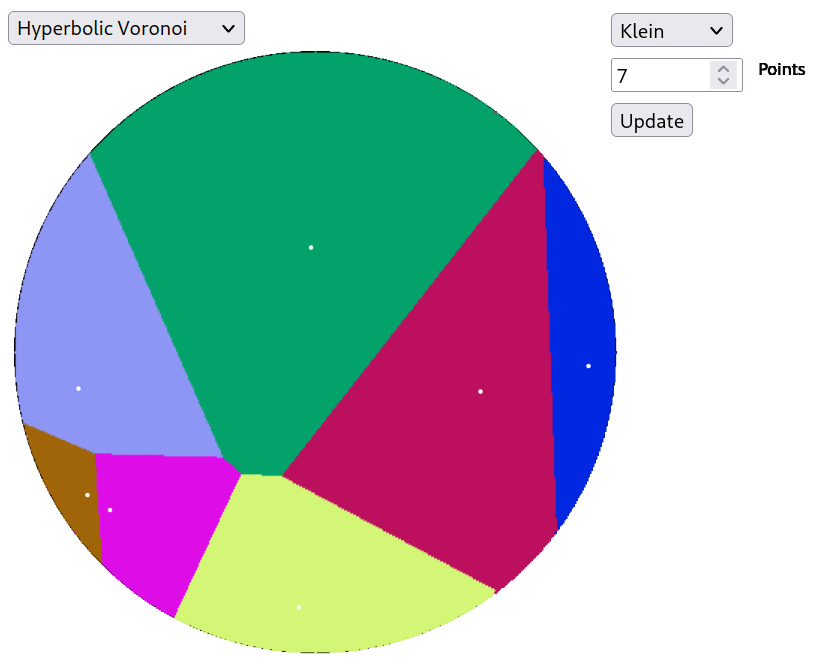
\includegraphics[scale=0.25]{k_voronoi_small.png}
	\end{figure}
	\begin{figure}[H]
		\centering
		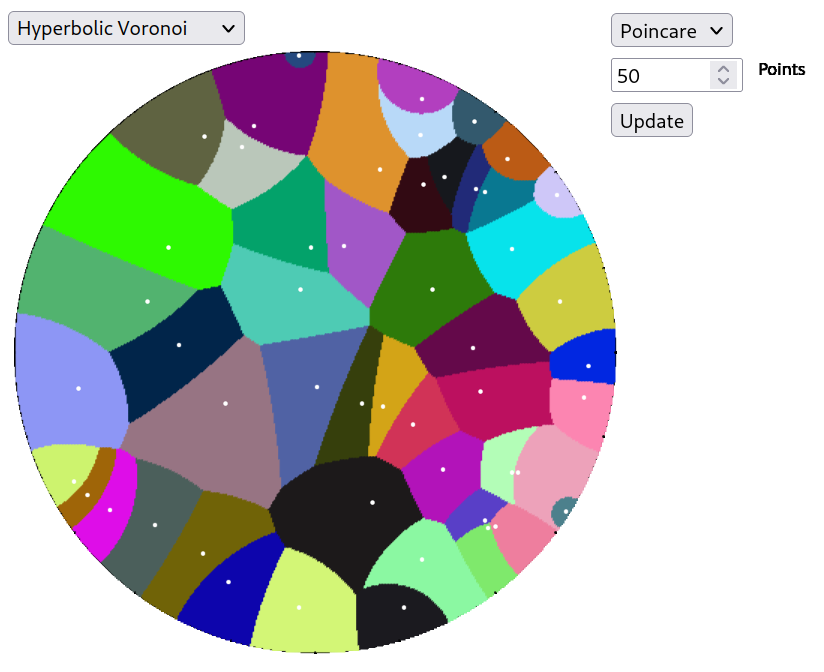
\includegraphics[scale=0.25]{p_voronoi_big.png}
		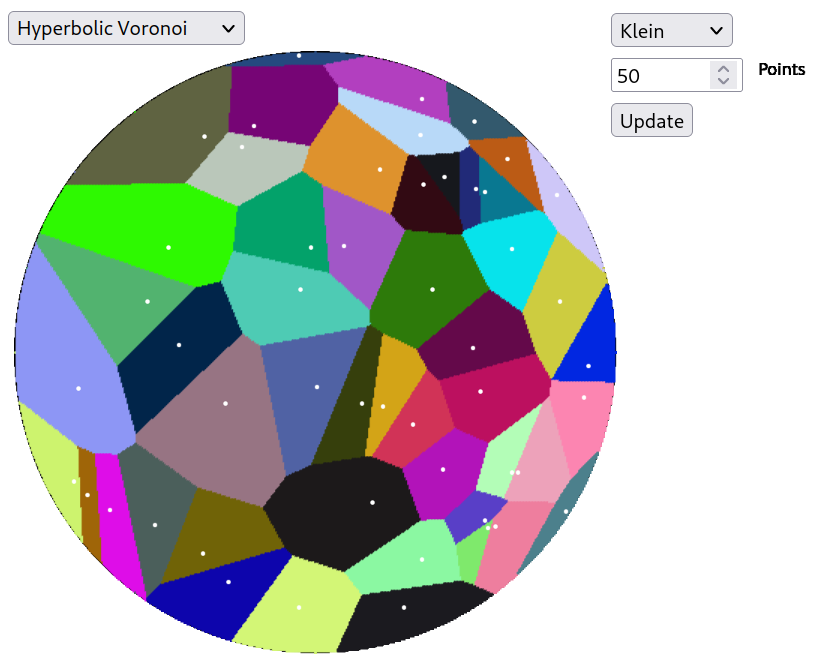
\includegraphics[scale=0.25]{k_voronoi_big.png}
	\end{figure}
\end{enumerate}

\bibliographystyle{unsrt}
\bibliography{refs}

\end{document}
